\documentclass{article}
\usepackage[margin=1in]{geometry}
\usepackage{amsmath,amsthm,amssymb}
\usepackage{bbm,enumerate,mathtools}
\usepackage{tikz,pgfplots}
\usepackage{chessboard}
\usepackage[hidelinks]{hyperref}
\usepackage{multicol} % Problem 35

\newenvironment{question}{\begin{trivlist}\item[\textbf{Question.}]}{\end{trivlist}}
\newenvironment{note}{\begin{trivlist}\item[\textbf{Note.}]}{\end{trivlist}}
\newenvironment{references}{\begin{trivlist}\item[\textbf{References.}]}{\end{trivlist}}
\newenvironment{related}{\begin{trivlist}\item[\textbf{Related.}]\end{trivlist}\begin{enumerate}}{\end{enumerate}}


\begin{document}

\rating{3}{2}
Consider maximal non-self-intersecting polygonal chains on $[n] \times [m]$
stable under $180^\circ$ rotation.

\begin{figure}[ht!]
  \centering
  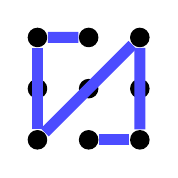
\begin{tikzpicture}[scale=0.65]
    \foreach \i in {1,2,3} {
      \foreach \j in {1,2,3} {
        \node[inner sep=2.5pt, circle, fill] (v\i\j) at ({\j-1},{3-\i}) {};
      }
    }
    \draw[line width=4, blue!70]
      (v12) edge (v11)
      (v11) edge (v31)
      (v31) edge (v13)
      (v13) edge (v33)
      (v33) edge (v32)
    ;
  \end{tikzpicture}
  ~
  
\begin{tikzpicture}[scale=0.65]
    \foreach \i in {1,2,3} {
      \foreach \j in {1,2,3} {
        \node[inner sep=2.5pt, circle, fill] (v\i\j) at ({\j-1},{3-\i}) {};
      }
    }
    \draw[line width=4, blue!70]
      (v21) edge (v11)
      (v11) edge (v12)
      (v12) edge (v31)
      (v31) edge (v13)
      (v13) edge (v32)
      (v32) edge (v33)
      (v33) edge (v23)
    ;
  \end{tikzpicture}
  ~
  
\begin{tikzpicture}[scale=0.65]
    \foreach \i in {1,2,3} {
      \foreach \j in {1,2,3} {
        \node[inner sep=2.5pt, circle, fill] (v\i\j) at ({\j-1},{3-\i}) {};
      }
    }
    \draw[line width=4, blue!70]
      (v11) edge (v21)
      (v21) edge (v12)
      (v12) edge (v31)
      (v31) edge (v13)
      (v13) edge (v32)
      (v32) edge (v23)
      (v23) edge (v33)
    ;
  \end{tikzpicture}
  ~
  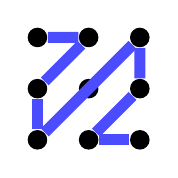
\begin{tikzpicture}[scale=0.65]
    \foreach \i in {1,2,3} {
      \foreach \j in {1,2,3} {
        \node[inner sep=2.5pt, circle, fill] (v\i\j) at ({\j-1},{3-\i}) {};
      }
    }
    \draw[line width=4, blue!70]
      (v11) edge (v12)
      (v12) edge (v21)
      (v21) edge (v31)
      (v31) edge (v13)
      (v13) edge (v23)
      (v23) edge (v32)
      (v32) edge (v33)
    ;
  \end{tikzpicture}
  ~
  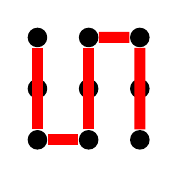
\begin{tikzpicture}[scale=0.65]
    \foreach \i in {1,2,3} {
      \foreach \j in {1,2,3} {
        \node[inner sep=2.5pt, circle, fill] (v\i\j) at ({\j-1},{3-\i}) {};
      }
    }
    \draw[line width=4, red]
      (v11) edge (v31)
      (v31) edge (v32)
      (v32) edge (v12)
      (v12) edge (v13)
      (v13) edge (v33)
    ;
  \end{tikzpicture}
  ~
  
\begin{tikzpicture}[scale=0.65]
    \foreach \i in {1,2,3} {
      \foreach \j in {1,2,3} {
        \node[inner sep=2.5pt, circle, fill] (v\i\j) at ({\j-1},{3-\i}) {};
      }
    }
    \draw[line width=4, red]
      (v11) edge (v31)
      (v31) edge (v12)
      (v12) edge (v32)
      (v32) edge (v13)
      (v13) edge (v33)
    ;
  \end{tikzpicture}
  ~
  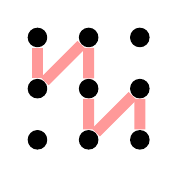
\begin{tikzpicture}[scale=0.65]
    \foreach \i in {1,2,3} {
      \foreach \j in {1,2,3} {
        \node[inner sep=2.5pt, circle, fill] (v\i\j) at ({\j-1},{3-\i}) {};
      }
    }
    \draw[line width=4, red!40]
      (v11) edge (v21)
      (v21) edge (v12)
      (v12) edge (v22)
      (v22) edge (v32)
      (v32) edge (v23)
      (v23) edge (v33)
    ;
  \end{tikzpicture}
  ~
  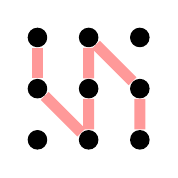
\begin{tikzpicture}[scale=0.65]
    \foreach \i in {1,2,3} {
      \foreach \j in {1,2,3} {
        \node[inner sep=2.5pt, circle, fill] (v\i\j) at ({\j-1},{3-\i}) {};
      }
    }
    \draw[line width=4, red!40]
      (v11) edge (v21)
      (v21) edge (v32)
      (v32) edge (v22)
      (v22) edge (v12)
      (v12) edge (v23)
      (v23) edge (v33)
    ;
  \end{tikzpicture}
  \caption{The $6$ (or $8$) maximal polygonal chains with vertices in $[3] \times [3]$.}
\end{figure}

\begin{figure}[ht!]
  \centering
  
\begin{tikzpicture}[scale=0.3] \draw (1,1)--(1,2)--(1,3)--(1,4)--(2,1)--(2,2)--(2,3)--(2,4)--(3,1)--(3,2)--(3,3)--(3,4); \end{tikzpicture} ~
  \begin{tikzpicture}[scale=0.3] \draw (1,1)--(1,2)--(1,3)--(1,4)--(2,4)--(2,3)--(2,2)--(2,1)--(3,1)--(3,2)--(3,3)--(3,4); \end{tikzpicture} ~
  
\begin{tikzpicture}[scale=0.3] \draw (1,1)--(1,2)--(1,3)--(2,1)--(1,4)--(2,2)--(2,3)--(3,1)--(2,4)--(3,2)--(3,3)--(3,4); \end{tikzpicture} ~
  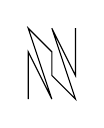
\begin{tikzpicture}[scale=0.3] \draw (1,1)--(1,2)--(1,3)--(2,1)--(1,4)--(2,3)--(2,2)--(3,1)--(2,4)--(3,2)--(3,3)--(3,4); \end{tikzpicture} ~
  
\begin{tikzpicture}[scale=0.3] \draw (1,1)--(1,2)--(1,3)--(2,1)--(2,2)--(1,4)--(3,1)--(2,3)--(2,4)--(3,2)--(3,3)--(3,4); \end{tikzpicture} ~
  
\begin{tikzpicture}[scale=0.3] \draw (1,1)--(1,2)--(1,3)--(2,1)--(2,2)--(3,1)--(1,4)--(2,3)--(2,4)--(3,2)--(3,3)--(3,4); \end{tikzpicture} ~
  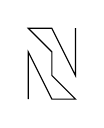
\begin{tikzpicture}[scale=0.3] \draw (1,1)--(1,2)--(1,3)--(2,1)--(3,1)--(2,2)--(2,3)--(1,4)--(2,4)--(3,2)--(3,3)--(3,4); \end{tikzpicture} ~
  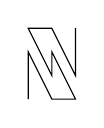
\begin{tikzpicture}[scale=0.3] \draw (1,1)--(1,2)--(1,3)--(2,1)--(3,1)--(2,3)--(2,2)--(1,4)--(2,4)--(3,2)--(3,3)--(3,4); \end{tikzpicture} ~
  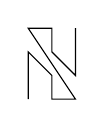
\begin{tikzpicture}[scale=0.3] \draw (1,1)--(1,2)--(1,3)--(2,2)--(2,1)--(3,1)--(1,4)--(2,4)--(2,3)--(3,2)--(3,3)--(3,4); \end{tikzpicture} ~
  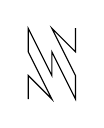
\begin{tikzpicture}[scale=0.3] \draw (1,1)--(1,2)--(2,1)--(1,3)--(1,4)--(2,2)--(2,3)--(3,1)--(3,2)--(2,4)--(3,3)--(3,4); \end{tikzpicture} ~
  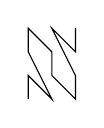
\begin{tikzpicture}[scale=0.3] \draw (1,1)--(1,2)--(2,1)--(1,3)--(1,4)--(2,3)--(2,2)--(3,1)--(3,2)--(2,4)--(3,3)--(3,4); \end{tikzpicture} ~
  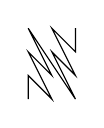
\begin{tikzpicture}[scale=0.3] \draw (1,1)--(1,2)--(2,1)--(1,3)--(2,2)--(1,4)--(3,1)--(2,3)--(3,2)--(2,4)--(3,3)--(3,4); \end{tikzpicture} ~
  
\begin{tikzpicture}[scale=0.3] \draw (1,1)--(1,2)--(2,1)--(1,3)--(2,2)--(3,1)--(1,4)--(2,3)--(3,2)--(2,4)--(3,3)--(3,4); \end{tikzpicture} ~
  
\begin{tikzpicture}[scale=0.3] \draw (1,1)--(1,2)--(2,1)--(2,2)--(1,3)--(1,4)--(3,1)--(3,2)--(2,3)--(2,4)--(3,3)--(3,4); \end{tikzpicture} ~
  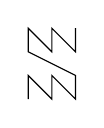
\begin{tikzpicture}[scale=0.3] \draw (1,1)--(1,2)--(2,1)--(2,2)--(3,1)--(3,2)--(1,3)--(1,4)--(2,3)--(2,4)--(3,3)--(3,4); \end{tikzpicture} ~
  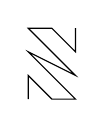
\begin{tikzpicture}[scale=0.3] \draw (1,1)--(1,2)--(2,1)--(3,1)--(2,2)--(1,3)--(3,2)--(2,3)--(1,4)--(2,4)--(3,3)--(3,4); \end{tikzpicture} ~
  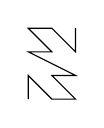
\begin{tikzpicture}[scale=0.3] \draw (1,1)--(1,2)--(2,1)--(3,1)--(2,2)--(3,2)--(1,3)--(2,3)--(1,4)--(2,4)--(3,3)--(3,4); \end{tikzpicture} \\~\\
  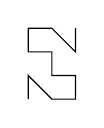
\begin{tikzpicture}[scale=0.3] \draw (1,1)--(1,2)--(2,1)--(3,1)--(3,2)--(2,2)--(2,3)--(1,3)--(1,4)--(2,4)--(3,3)--(3,4); \end{tikzpicture} ~
  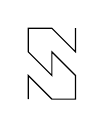
\begin{tikzpicture}[scale=0.3] \draw (1,1)--(1,2)--(2,1)--(3,1)--(3,2)--(2,3)--(2,2)--(1,3)--(1,4)--(2,4)--(3,3)--(3,4); \end{tikzpicture} ~
  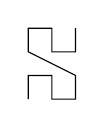
\begin{tikzpicture}[scale=0.3] \draw (1,1)--(1,2)--(2,2)--(2,1)--(3,1)--(3,2)--(1,3)--(1,4)--(2,4)--(2,3)--(3,3)--(3,4); \end{tikzpicture} ~
  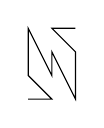
\begin{tikzpicture}[scale=0.3] \draw (1,1)--(2,1)--(1,2)--(1,3)--(1,4)--(2,2)--(2,3)--(3,1)--(3,2)--(3,3)--(2,4)--(3,4); \end{tikzpicture} ~
  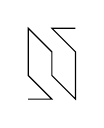
\begin{tikzpicture}[scale=0.3] \draw (1,1)--(2,1)--(1,2)--(1,3)--(1,4)--(2,3)--(2,2)--(3,1)--(3,2)--(3,3)--(2,4)--(3,4); \end{tikzpicture} ~
  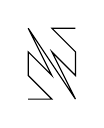
\begin{tikzpicture}[scale=0.3] \draw (1,1)--(2,1)--(1,2)--(1,3)--(2,2)--(1,4)--(3,1)--(2,3)--(3,2)--(3,3)--(2,4)--(3,4); \end{tikzpicture} ~
  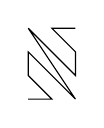
\begin{tikzpicture}[scale=0.3] \draw (1,1)--(2,1)--(1,2)--(1,3)--(2,2)--(3,1)--(1,4)--(2,3)--(3,2)--(3,3)--(2,4)--(3,4); \end{tikzpicture} ~
  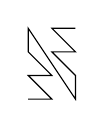
\begin{tikzpicture}[scale=0.3] \draw (1,1)--(2,1)--(1,2)--(2,2)--(1,3)--(1,4)--(3,1)--(3,2)--(2,3)--(3,3)--(2,4)--(3,4); \end{tikzpicture} ~
  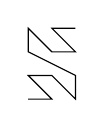
\begin{tikzpicture}[scale=0.3] \draw (1,1)--(2,1)--(1,2)--(2,2)--(3,1)--(3,2)--(1,3)--(1,4)--(2,3)--(3,3)--(2,4)--(3,4); \end{tikzpicture} ~
  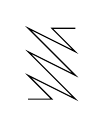
\begin{tikzpicture}[scale=0.3] \draw (1,1)--(2,1)--(1,2)--(3,1)--(2,2)--(1,3)--(3,2)--(2,3)--(1,4)--(3,3)--(2,4)--(3,4); \end{tikzpicture} ~
  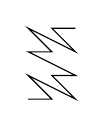
\begin{tikzpicture}[scale=0.3] \draw (1,1)--(2,1)--(1,2)--(3,1)--(2,2)--(3,2)--(1,3)--(2,3)--(1,4)--(3,3)--(2,4)--(3,4); \end{tikzpicture} ~
  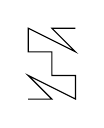
\begin{tikzpicture}[scale=0.3] \draw (1,1)--(2,1)--(1,2)--(3,1)--(3,2)--(2,2)--(2,3)--(1,3)--(1,4)--(3,3)--(2,4)--(3,4); \end{tikzpicture} ~
  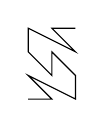
\begin{tikzpicture}[scale=0.3] \draw (1,1)--(2,1)--(1,2)--(3,1)--(3,2)--(2,3)--(2,2)--(1,3)--(1,4)--(3,3)--(2,4)--(3,4); \end{tikzpicture} ~
  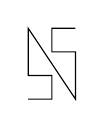
\begin{tikzpicture}[scale=0.3] \draw (1,1)--(2,1)--(2,2)--(1,2)--(1,3)--(1,4)--(3,1)--(3,2)--(3,3)--(2,3)--(2,4)--(3,4); \end{tikzpicture} ~
  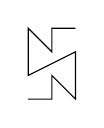
\begin{tikzpicture}[scale=0.3] \draw (1,1)--(2,1)--(2,2)--(3,1)--(3,2)--(3,3)--(1,2)--(1,3)--(1,4)--(2,3)--(2,4)--(3,4); \end{tikzpicture} ~
  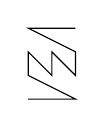
\begin{tikzpicture}[scale=0.3] \draw (1,1)--(2,1)--(3,1)--(1,2)--(1,3)--(2,2)--(2,3)--(3,2)--(3,3)--(1,4)--(2,4)--(3,4); \end{tikzpicture} ~
  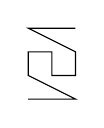
\begin{tikzpicture}[scale=0.3] \draw (1,1)--(2,1)--(3,1)--(1,2)--(1,3)--(2,3)--(2,2)--(3,2)--(3,3)--(1,4)--(2,4)--(3,4); \end{tikzpicture} \\~\\
  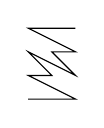
\begin{tikzpicture}[scale=0.3] \draw (1,1)--(2,1)--(3,1)--(1,2)--(2,2)--(1,3)--(3,2)--(2,3)--(3,3)--(1,4)--(2,4)--(3,4); \end{tikzpicture} ~
  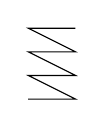
\begin{tikzpicture}[scale=0.3] \draw (1,1)--(2,1)--(3,1)--(1,2)--(2,2)--(3,2)--(1,3)--(2,3)--(3,3)--(1,4)--(2,4)--(3,4); \end{tikzpicture} ~
  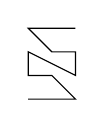
\begin{tikzpicture}[scale=0.3] \draw (1,1)--(2,1)--(3,1)--(2,2)--(1,2)--(1,3)--(3,2)--(3,3)--(2,3)--(1,4)--(2,4)--(3,4); \end{tikzpicture} ~
  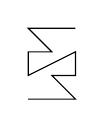
\begin{tikzpicture}[scale=0.3] \draw (1,1)--(2,1)--(3,1)--(2,2)--(3,2)--(3,3)--(1,2)--(1,3)--(2,3)--(1,4)--(2,4)--(3,4); \end{tikzpicture} ~
  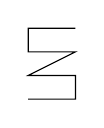
\begin{tikzpicture}[scale=0.3] \draw (1,1)--(2,1)--(3,1)--(3,2)--(2,2)--(1,2)--(3,3)--(2,3)--(1,3)--(1,4)--(2,4)--(3,4); \end{tikzpicture} ~
  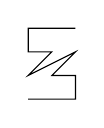
\begin{tikzpicture}[scale=0.3] \draw (1,1)--(2,1)--(3,1)--(3,2)--(2,2)--(3,3)--(1,2)--(2,3)--(1,3)--(1,4)--(2,4)--(3,4); \end{tikzpicture} ~
  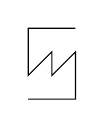
\begin{tikzpicture}[scale=0.3] \draw (1,1)--(2,1)--(3,1)--(3,2)--(3,3)--(2,2)--(2,3)--(1,2)--(1,3)--(1,4)--(2,4)--(3,4); \end{tikzpicture} ~
  \begin{tikzpicture}[scale=0.3] \draw (1,1)--(2,1)--(3,1)--(3,2)--(3,3)--(2,3)--(2,2)--(1,2)--(1,3)--(1,4)--(2,4)--(3,4); \end{tikzpicture} ~
  \begin{tikzpicture}[scale=0.3] \draw (1,1)--(2,2)--(2,1)--(3,1)--(3,2)--(3,3)--(1,2)--(1,3)--(1,4)--(2,4)--(2,3)--(3,4); \end{tikzpicture} ~
  \begin{tikzpicture}[scale=0.3] \draw (1,2)--(1,1)--(2,1)--(1,3)--(1,4)--(2,2)--(2,3)--(3,1)--(3,2)--(2,4)--(3,4)--(3,3); \end{tikzpicture} ~
  \begin{tikzpicture}[scale=0.3] \draw (1,2)--(1,1)--(2,1)--(1,3)--(1,4)--(2,3)--(2,2)--(3,1)--(3,2)--(2,4)--(3,4)--(3,3); \end{tikzpicture} ~
  \begin{tikzpicture}[scale=0.3] \draw (1,2)--(1,1)--(2,1)--(1,3)--(2,2)--(1,4)--(3,1)--(2,3)--(3,2)--(2,4)--(3,4)--(3,3); \end{tikzpicture} ~
  \begin{tikzpicture}[scale=0.3] \draw (1,2)--(1,1)--(2,1)--(1,3)--(2,2)--(3,1)--(1,4)--(2,3)--(3,2)--(2,4)--(3,4)--(3,3); \end{tikzpicture} ~
  \begin{tikzpicture}[scale=0.3] \draw (1,2)--(1,1)--(2,1)--(2,2)--(1,3)--(1,4)--(3,1)--(3,2)--(2,3)--(2,4)--(3,4)--(3,3); \end{tikzpicture} ~
  \begin{tikzpicture}[scale=0.3] \draw (1,2)--(1,1)--(2,1)--(2,2)--(3,1)--(3,2)--(1,3)--(1,4)--(2,3)--(2,4)--(3,4)--(3,3); \end{tikzpicture} ~
  \begin{tikzpicture}[scale=0.3] \draw (1,2)--(1,1)--(2,1)--(3,1)--(2,2)--(1,3)--(3,2)--(2,3)--(1,4)--(2,4)--(3,4)--(3,3); \end{tikzpicture} ~
  \begin{tikzpicture}[scale=0.3] \draw (1,2)--(1,1)--(2,1)--(3,1)--(2,2)--(3,2)--(1,3)--(2,3)--(1,4)--(2,4)--(3,4)--(3,3); \end{tikzpicture} \\~\\
  \begin{tikzpicture}[scale=0.3] \draw (1,2)--(1,1)--(2,1)--(3,1)--(3,2)--(2,2)--(2,3)--(1,3)--(1,4)--(2,4)--(3,4)--(3,3); \end{tikzpicture} ~
  \begin{tikzpicture}[scale=0.3] \draw (1,2)--(1,1)--(2,1)--(3,1)--(3,2)--(2,3)--(2,2)--(1,3)--(1,4)--(2,4)--(3,4)--(3,3); \end{tikzpicture} ~
  \begin{tikzpicture}[scale=0.3] \draw (1,2)--(1,1)--(2,2)--(2,1)--(3,1)--(3,2)--(1,3)--(1,4)--(2,4)--(2,3)--(3,4)--(3,3); \end{tikzpicture} ~
  \begin{tikzpicture}[scale=0.3] \draw (1,2)--(1,3)--(1,4)--(2,3)--(2,4)--(3,4)--(1,1)--(2,1)--(2,2)--(3,1)--(3,2)--(3,3); \end{tikzpicture} ~
  \begin{tikzpicture}[scale=0.3] \draw (1,2)--(1,3)--(1,4)--(2,4)--(1,1)--(2,2)--(2,3)--(3,4)--(2,1)--(3,1)--(3,2)--(3,3); \end{tikzpicture} ~
  \begin{tikzpicture}[scale=0.3] \draw (1,2)--(1,3)--(1,4)--(2,4)--(1,1)--(2,3)--(2,2)--(3,4)--(2,1)--(3,1)--(3,2)--(3,3); \end{tikzpicture} ~
  \begin{tikzpicture}[scale=0.3] \draw (1,2)--(1,3)--(1,4)--(2,4)--(2,3)--(1,1)--(3,4)--(2,2)--(2,1)--(3,1)--(3,2)--(3,3); \end{tikzpicture} ~
  \begin{tikzpicture}[scale=0.3] \draw (1,2)--(1,3)--(1,4)--(2,4)--(2,3)--(3,4)--(1,1)--(2,2)--(2,1)--(3,1)--(3,2)--(3,3); \end{tikzpicture} ~
  \begin{tikzpicture}[scale=0.3] \draw (1,2)--(1,3)--(1,4)--(2,4)--(3,4)--(2,2)--(2,3)--(1,1)--(2,1)--(3,1)--(3,2)--(3,3); \end{tikzpicture} ~
  \begin{tikzpicture}[scale=0.3] \draw (1,2)--(1,3)--(1,4)--(2,4)--(3,4)--(2,3)--(2,2)--(1,1)--(2,1)--(3,1)--(3,2)--(3,3); \end{tikzpicture} ~
  \begin{tikzpicture}[scale=0.3] \draw (1,2)--(1,3)--(2,2)--(1,1)--(2,1)--(3,1)--(1,4)--(2,4)--(3,4)--(2,3)--(3,2)--(3,3); \end{tikzpicture} ~
  \begin{tikzpicture}[scale=0.3] \draw (1,2)--(1,3)--(2,3)--(1,4)--(2,4)--(3,4)--(1,1)--(2,1)--(3,1)--(2,2)--(3,2)--(3,3); \end{tikzpicture} ~
  \begin{tikzpicture}[scale=0.3] \draw (1,2)--(2,2)--(1,1)--(2,1)--(3,1)--(3,2)--(1,3)--(1,4)--(2,4)--(3,4)--(2,3)--(3,3); \end{tikzpicture} ~
  \begin{tikzpicture}[scale=0.3] \draw (1,2)--(2,3)--(1,3)--(1,4)--(2,4)--(3,4)--(1,1)--(2,1)--(3,1)--(3,2)--(2,2)--(3,3); \end{tikzpicture} ~
  \begin{tikzpicture}[scale=0.3] \draw (2,1)--(1,1)--(1,2)--(1,3)--(1,4)--(2,2)--(2,3)--(3,1)--(3,2)--(3,3)--(3,4)--(2,4); \end{tikzpicture} ~
  \begin{tikzpicture}[scale=0.3] \draw (2,1)--(1,1)--(1,2)--(1,3)--(1,4)--(2,3)--(2,2)--(3,1)--(3,2)--(3,3)--(3,4)--(2,4); \end{tikzpicture} ~
  \begin{tikzpicture}[scale=0.3] \draw (2,1)--(1,1)--(1,2)--(1,3)--(2,2)--(1,4)--(3,1)--(2,3)--(3,2)--(3,3)--(3,4)--(2,4); \end{tikzpicture} \\~\\
  \begin{tikzpicture}[scale=0.3] \draw (2,1)--(1,1)--(1,2)--(1,3)--(2,2)--(3,1)--(1,4)--(2,3)--(3,2)--(3,3)--(3,4)--(2,4); \end{tikzpicture} ~
  \begin{tikzpicture}[scale=0.3] \draw (2,1)--(1,1)--(1,2)--(2,2)--(1,3)--(1,4)--(3,1)--(3,2)--(2,3)--(3,3)--(3,4)--(2,4); \end{tikzpicture} ~
  \begin{tikzpicture}[scale=0.3] \draw (2,1)--(1,1)--(1,2)--(2,2)--(3,1)--(3,2)--(1,3)--(1,4)--(2,3)--(3,3)--(3,4)--(2,4); \end{tikzpicture} ~
  \begin{tikzpicture}[scale=0.3] \draw (2,1)--(1,1)--(1,2)--(3,1)--(2,2)--(1,3)--(3,2)--(2,3)--(1,4)--(3,3)--(3,4)--(2,4); \end{tikzpicture} ~
  \begin{tikzpicture}[scale=0.3] \draw (2,1)--(1,1)--(1,2)--(3,1)--(2,2)--(3,2)--(1,3)--(2,3)--(1,4)--(3,3)--(3,4)--(2,4); \end{tikzpicture} ~
  \begin{tikzpicture}[scale=0.3] \draw (2,1)--(1,1)--(1,2)--(3,1)--(3,2)--(2,2)--(2,3)--(1,3)--(1,4)--(3,3)--(3,4)--(2,4); \end{tikzpicture} ~
  \begin{tikzpicture}[scale=0.3] \draw (2,1)--(1,1)--(1,2)--(3,1)--(3,2)--(2,3)--(2,2)--(1,3)--(1,4)--(3,3)--(3,4)--(2,4); \end{tikzpicture} ~
  \begin{tikzpicture}[scale=0.3] \draw (2,1)--(1,1)--(2,2)--(1,2)--(1,3)--(1,4)--(3,1)--(3,2)--(3,3)--(2,3)--(3,4)--(2,4); \end{tikzpicture} ~
  \begin{tikzpicture}[scale=0.3] \draw (2,1)--(1,1)--(2,2)--(3,1)--(3,2)--(3,3)--(1,2)--(1,3)--(1,4)--(2,3)--(3,4)--(2,4); \end{tikzpicture} ~
  \begin{tikzpicture}[scale=0.3] \draw (2,1)--(2,2)--(1,1)--(1,2)--(1,3)--(1,4)--(3,1)--(3,2)--(3,3)--(3,4)--(2,3)--(2,4); \end{tikzpicture} ~
  \begin{tikzpicture}[scale=0.3] \draw (2,2)--(1,1)--(2,1)--(3,1)--(3,2)--(3,3)--(1,2)--(1,3)--(1,4)--(2,4)--(3,4)--(2,3); \end{tikzpicture} ~
  \begin{tikzpicture}[scale=0.3] \draw (2,2)--(1,2)--(1,1)--(2,1)--(3,1)--(3,2)--(1,3)--(1,4)--(2,4)--(3,4)--(3,3)--(2,3); \end{tikzpicture} ~
  \begin{tikzpicture}[scale=0.3] \draw (2,2)--(1,3)--(1,2)--(1,1)--(2,1)--(3,1)--(1,4)--(2,4)--(3,4)--(3,3)--(3,2)--(2,3); \end{tikzpicture} ~
  \begin{tikzpicture}[scale=0.3] \draw (2,2)--(2,1)--(1,1)--(1,2)--(1,3)--(1,4)--(3,1)--(3,2)--(3,3)--(3,4)--(2,4)--(2,3); \end{tikzpicture}
  \caption{$f(4 \times 3) = 82$}
\end{figure}

\begin{question}
  How many non-self-intersecting polygonal chains with vertex set equal to
  $[n] \times [m]$ are stable under $180^\circ$ rotation?
\end{question}

\begin{related}
  \item What if this is done with other kinds of symmetry?
  (e.g. horizontal or vertical reflection)
  \item What if this is done for polygons instead of polygonal chains?
  \item What if maximal means that the polygonal chain cannot be extended, a
  weaker condition than that the vertex set is $[n] \times [m]$.
  (This includes the last two chains in the example.)
  \item What is the maximal length of such a chain with respect to
    $\ell_1, \ell_2,$ and $\ell_\infty$?
    What if the symmetry restriction is dropped?
  \item What if the only allowed moves are king moves? Rook moves?
  \item What if this is done with vertex set
    $[n_1] \times [n_2] \times \cdots \times [n_k]$?
\end{related}

\begin{references}
  \item Problems 5, 44, 46, 55, 68, 74, 87, and 104.
\end{references}
\end{document}
